\section{Data Architecture}

%%% Texto introductorio :p

%%%%% DE AQUI EN ADELANTE OTRA VEZ POR FRENTE xD
\subsection{Storage Type}

% ------------------------- Payments and Refunds -------------------------
\begingroup
\setlength{\emergencystretch}{3em}
\subsubsection{Payments and Refunds}
\label{sec:pay-storage}

\begin{longtable}{@{}L{3.4cm}L{3.0cm}L{7.4cm}@{}}
\toprule
\textbf{Data} & \textbf{Storage} & \textbf{Rationale} \\
\midrule
\endhead
Payments, attempts, refunds & Relational, Payment Coordination &
  Structured records with rules the database must enforce: one payment per
  reservation (unique) and refunded amount $\leq$ captured amount (check).
  Low write volume (5\,\% of the traffic). \\
Idempotency records & Relational (same database) &
  Written in the same transaction as the payment change, so a retry can never
  charge twice. A cache is not used because it can lose keys, the same choice
  Airbnb made for its payments~\cite{airbnb-orpheus}. \\
Inbox and outbox & Relational (same database) &
  The inbox removes duplicate webhooks; the outbox publishes events without
  dual writes. \\
Ledger (accounts, journal, entries) & Relational, Ledger \& Payout &
  Append-only; every journal transaction must balance (debits = credits);
  auditors need joins and totals. \\
Host payouts & Relational (same ledger database) &
  Small transactional table with a unique key per payout. \\
\bottomrule
\caption{Storage of the Payments and Refunds work stream.}
\label{tab:pay-storage}
\end{longtable}

Money is stored as an \textbf{integer amount plus a currency code} (e.g.\
\texttt{1070000}, \texttt{COP}), never as a decimal number, so rounding can
never create or lose money.
\endgroup

\subsubsection{Reservation and Calendar }
A single \textbf{relational PostgreSQL} database holds accommodations,
calendar, reservations, agreements and outbox: the exclusion constraint and the
reservation change must commit in the same transaction. No cache sits in front
of availability. Hold timers live in the scheduler and are rebuildable from
\texttt{hold\_expires\_at}.

% ------------------------- Pricing Engine -------------------------
\begingroup
\setlength{\emergencystretch}{3em}
\subsubsection{Pricing Engine}
\label{sec:price-storage}

\begin{longtable}{@{}L{3.4cm}L{3.2cm}L{7.2cm}@{}}
\toprule
\textbf{Data} & \textbf{Storage} & \textbf{Rationale} \\
\midrule
\endhead
Model versions, zone snapshot & Relational, Pricing Service &
  Small tables with rules the database must enforce: exactly one
  \texttt{ACTIVE} version (partial unique index) and one snapshot row per
  zone. The multiplier request is a single key read. \\
Calculation history & Document store, Pricing Service &
  Append-only, one self-contained document per calculation (inputs,
  indicators, result); read by listing and time range. \\
History older than one year & Object storage &
  Cheap columnar files for audit and for training the next model version. \\
Search counters, demand snapshots & Key-value / time-series, Demand
  Indicators & High write rate (one increment per search event) on keys
  \texttt{zone\_id\#day}; derived data that can be rebuilt. \\
Fetch runs, context events & Relational, Context Indicators &
  Low volume, monthly batch; a unique key avoids duplicate events when a run
  is repeated. \\
\bottomrule
\caption{Storage of the Pricing Engine work stream.}
\label{tab:price-storage}
\end{longtable}
\endgroup

% ------------------------- Identity, Communication and Internal Operations -------------------------
\begingroup
\setlength{\emergencystretch}{3em}
\subsubsection{Identity, Communication and Internal Operations}
\label{sec:id-storage}

\begin{longtable}{@{}L{3.5cm}L{3.1cm}L{7.2cm}@{}}
\toprule
\textbf{Data} & \textbf{Storage} & \textbf{Rationale} \\
\midrule
\endhead
Credentials, MFA factors, sessions, signing keys, revocations &
  Dedicated identity store, Identity \& Access &
  Keeps password material out of application databases, supports key
  rotation and immediate session revocation. \\
Profiles, role assignments, account status & Relational, User Profile &
  Strong integrity and transactional role changes; administrative queries
  over related records. \\
Conversations, messages, read state & Document or wide-column store,
  Messaging &
  High write and read volume, per-conversation ordering and horizontal
  partitioning by \texttt{conversationId}. \\
Attachment content & Object storage, Messaging &
  Large binary objects stay out of the database and are served through
  short-lived URLs. \\
Preferences, devices, delivery attempts, processed events &
  Key-value or document store, Notification &
  Point lookups by user, device or event; expiry (TTL) of the
  duplicate-suppression keys. \\
Support cases, comments, transitions & Relational, Support &
  Related records, ordered transitions and queries by status, assignee and
  related entity. \\
Administrative actions, approvals, policies & Relational, Administration &
  Transactional workflow state and clear relations between an action, its
  approvals and its outcome. \\
Audit records and anchors & Append-only immutable store, Audit &
  Tamper-evident retention, independent verification, no update or delete. \\
Audit search index & Search index, Audit &
  Derived and rebuildable projection for read-only queries. \\
Logs, metrics, traces & Observability platform &
  Operational diagnosis only; never accepted as audit evidence. \\
\bottomrule
\caption{Storage of the Identity, Communication and Internal Operations work
stream.}
\label{tab:id-storage}
\end{longtable}

Each service has its own database, schema and credentials. Passwords are
stored only as salted hashes; full message bodies and payment data never
appear in events, logs or audit payloads.
\endgroup

\subsection{Data model}

% ------------------------- Payments and Refunds -------------------------
\begingroup
\setlength{\emergencystretch}{3em}
\subsubsection{Payments and Refunds}
\label{sec:pay-model}

\begin{longtable}{@{}L{3.6cm}L{10.2cm}@{}}
\toprule
\textbf{Table} & \textbf{Main columns and constraints} \\
\midrule
\endhead
\multicolumn{2}{@{}l}{\emph{Payments DB (Payment Coordination)}} \\
\texttt{payment} & \texttt{payment\_id} (PK), \texttt{reservation\_\allowbreak id}
  (unique), \texttt{guest\_id}, \texttt{host\_id}, \texttt{amount},
  \texttt{captured\_\allowbreak amount}, \texttt{refunded\_\allowbreak amount} (check
  $\leq$ captured), \texttt{currency}, \texttt{price\_\allowbreak snapshot},
  \texttt{status}, \texttt{gateway\_\allowbreak reference}, \texttt{version}. \\
\texttt{payment\_\allowbreak attempt} & \texttt{attempt\_id} (PK, also the gateway
  idempotency key), \texttt{payment\_id} (FK), \texttt{attempt\_no},
  \texttt{method\_token}, \texttt{status}, \texttt{decline\_code}. \\
\texttt{refund} & \texttt{refund\_id} (PK), \texttt{payment\_id} (FK),
  \texttt{amount}, \texttt{reason}, \texttt{source} (\texttt{CANCELLATION},
  \texttt{SUPPORT}), \texttt{support\_\allowbreak case\_\allowbreak id}, \texttt{funded\_by},
  \texttt{status}, \texttt{idempotency\_\allowbreak key} (unique). \\
\texttt{idempotency\_\allowbreak record} & \texttt{idempotency\_\allowbreak key} (PK),
  \texttt{request\_hash}, \texttt{state} (\texttt{IN\_PROGRESS},
  \texttt{DONE}), \texttt{response\_\allowbreak code}, \texttt{response\_\allowbreak body},
  \texttt{expires\_at}. \\
\texttt{gateway\_\allowbreak event\_\allowbreak inbox}, \texttt{outbox\_event}, \texttt{processed\_\allowbreak event} &
  Received webhooks keyed by the gateway event id; outbox
  (\texttt{event\_id}, \texttt{type}, \texttt{payload},
  \texttt{published\_at}); processed events keyed by (\texttt{event\_id},
  \texttt{consumer}). \\
\addlinespace
\multicolumn{2}{@{}l}{\emph{Ledger DB (Ledger \& Payout)}} \\
\texttt{account} & \texttt{account\_id} (PK), \texttt{type}
  (\texttt{GATEWAY\_\allowbreak CLEARING}, \texttt{HOST\_PAYABLE},
  \texttt{PLATFORM\_\allowbreak MARGIN}, \texttt{GOODWILL\_\allowbreak EXPENSE}),
  \texttt{owner\_id} (host or null), \texttt{currency}. \\
\texttt{journal\_txn} & \texttt{txn\_id} (PK), \texttt{source\_\allowbreak event\_\allowbreak id}
  (unique), \texttt{type} (\texttt{CAPTURE}, \texttt{REFUND},
  \texttt{PAYOUT}), \texttt{reservation\_\allowbreak id}, \texttt{occurred\_at}. \\
\texttt{ledger\_entry} & \texttt{entry\_id} (PK), \texttt{txn\_id} (FK),
  \texttt{account\_id} (FK), \texttt{direction} (\texttt{DEBIT},
  \texttt{CREDIT}), \texttt{amount}. Append-only; debits equal credits per
  transaction. \\
\texttt{payout} & \texttt{payout\_id} (PK), \texttt{host\_id},
  \texttt{reservation\_\allowbreak id}, \texttt{amount}, \texttt{release\_at},
  \texttt{status} (\texttt{SCHEDULED}, \texttt{RELEASED}, \texttt{FAILED}),
  \texttt{idempotency\_\allowbreak key} (unique). \\
\bottomrule
\caption{Main tables of Payments and Refunds. \texttt{reservation\_\allowbreak id},
\texttt{guest\_id} and \texttt{host\_id} are logical references (no
cross-service foreign keys).}
\label{tab:pay-model}
\end{longtable}

\paragraph{How the money is split.} The guest is charged \textbf{once} for the
total. The split uses the \texttt{price\_\allowbreak snapshot} frozen by the
Reservation Service, where the multiplier from the Pricing work stream is the
platform margin (1.02, 1.07 or 1.15):
\[
  \textit{HostAmount} = \textit{basePrice} \times \textit{nights}
\]
\[
  \textit{PlatformMargin} = (\textit{multiplier} - 1) \times \textit{basePrice} \times \textit{nights}
\]
For the reservation \texttt{res-9f3a21} of the Reservation work stream
(4 nights, base price 250{,}000 COP, multiplier 1.07, cleaning included in the
base price), the guest pays 1{,}070{,}000 COP: 1{,}000{,}000 are owed to the
host and 70{,}000 are the platform margin.

\paragraph{Payment request (from the Reservation Service).}
{\footnotesize
\begin{verbatim}
POST /api/v1/payments
Idempotency-Key: book:res-9f3a21:auth:1
{ "reservationId": "res-9f3a21", "guestId": "guest-204",
  "hostId": "host-678", "amount": 1070000, "currency": "COP",
  "priceSnapshot": { "basePrice": 250000, "multiplier": 1.07,
                     "includesCleaning": true, "nights": 4,
                     "effectivePricePerNight": 267500 },
  "paymentMethodToken": "tok_7Hq2Lx" }
\end{verbatim}
}

\paragraph{Journal transaction written after the capture.}
{\footnotesize
\begin{verbatim}
{ "txn_id": "jt-10044", "source_event_id": "e-7c22d1",
  "type": "CAPTURE", "reservation_id": "res-9f3a21", "currency": "COP",
  "entries": [
  {"account":"GATEWAY_CLEARING","direction":"DEBIT","amount":1070000},
  {"account":"HOST_PAYABLE:host-678","direction":"CREDIT","amount":1000000},
  {"account":"PLATFORM_MARGIN","direction":"CREDIT","amount":70000} ] }
\end{verbatim}
}

A refund is a new transaction in the opposite direction. A refund funded by
the platform debits \texttt{GOODWILL\_\allowbreak EXPENSE} instead of the host's account.
A refund after the payout leaves the host's account negative, and the debt is
recovered from later payouts.
\endgroup

\subsubsection{Reservation and Calendar}
\begin{table}[!ht]
  \centering
  \small
  \begin{tabularx}{\textwidth}{@{}>{\raggedright\arraybackslash}p{5cm}>{\raggedright\arraybackslash}X@{}}
    \toprule
    \textbf{Table} & \textbf{Main columns} \\
    \midrule
    \texttt{accommodation} & \texttt{listing\_id} (PK), \texttt{host\_id}, \texttt{zone\_id}, \texttt{max\_guests}, \texttt{base\_price}, \texttt{includes\_cleaning}, \texttt{multiplier}, \texttt{effective\_nightly\_rate}, \texttt{status} (\texttt{ACTIVE}, \texttt{PAUSED}), \texttt{status\_reason}, \texttt{version} \\
    \texttt{reservation} & \texttt{reservation\_id} (PK), \texttt{listing\_id} (FK), \texttt{zone\_id}, \texttt{guest\_id}, \texttt{start\_date}, \texttt{end\_date}, \texttt{guests\_count}, \texttt{status}, \texttt{hold\_expires\_at}, \texttt{total\_amount}, \texttt{price\_snapshot}, \texttt{review\_reason}, \texttt{idempotency\_key}, \texttt{version} \\
    \texttt{calendar\_entry} & \texttt{entry\_id} (PK), \texttt{listing\_id} (FK), \texttt{zone\_id}, \texttt{period} (\texttt{daterange}), \texttt{kind} (\texttt{HOLD}, \texttt{RESERVATION}, \texttt{HOST\_BLOCK}), \texttt{reservation\_id} (FK), \texttt{expires\_at}, \texttt{released\_at} \\
    \texttt{checkin\_agreement} & \texttt{agreement\_id} (PK), \texttt{reservation\_id} (FK, unique), check-in/out times, \texttt{status}, acceptance timestamps \\
    \texttt{reservation\_status\_history} & \texttt{reservation\_id} (FK), \texttt{from\_status}, \texttt{to\_status}, \texttt{actor}, \texttt{reason} \\
    \texttt{outbox\_event}, \texttt{processed\_event} & Outbox (\texttt{event\_id}, \texttt{type}, \texttt{payload}, \texttt{published\_at}); (\texttt{event\_id}, \texttt{consumer}) for idempotency \\
    \bottomrule
  \end{tabularx}
  \caption{Data model of the Reservation and Accommodation Service.}
\end{table}
\noindent Reservation states: \texttt{PENDING\_PAYMENT}, \texttt{CONFIRMED},
\texttt{PAYMENT\_FAILED}, \texttt{EXPIRED}, \texttt{CANCELLED},


% ------------------------- Pricing Engine -------------------------
\begingroup
\setlength{\emergencystretch}{3em}
\subsubsection{Pricing Engine}
\label{sec:price-model}

\begin{figure}[H]
  \centering
  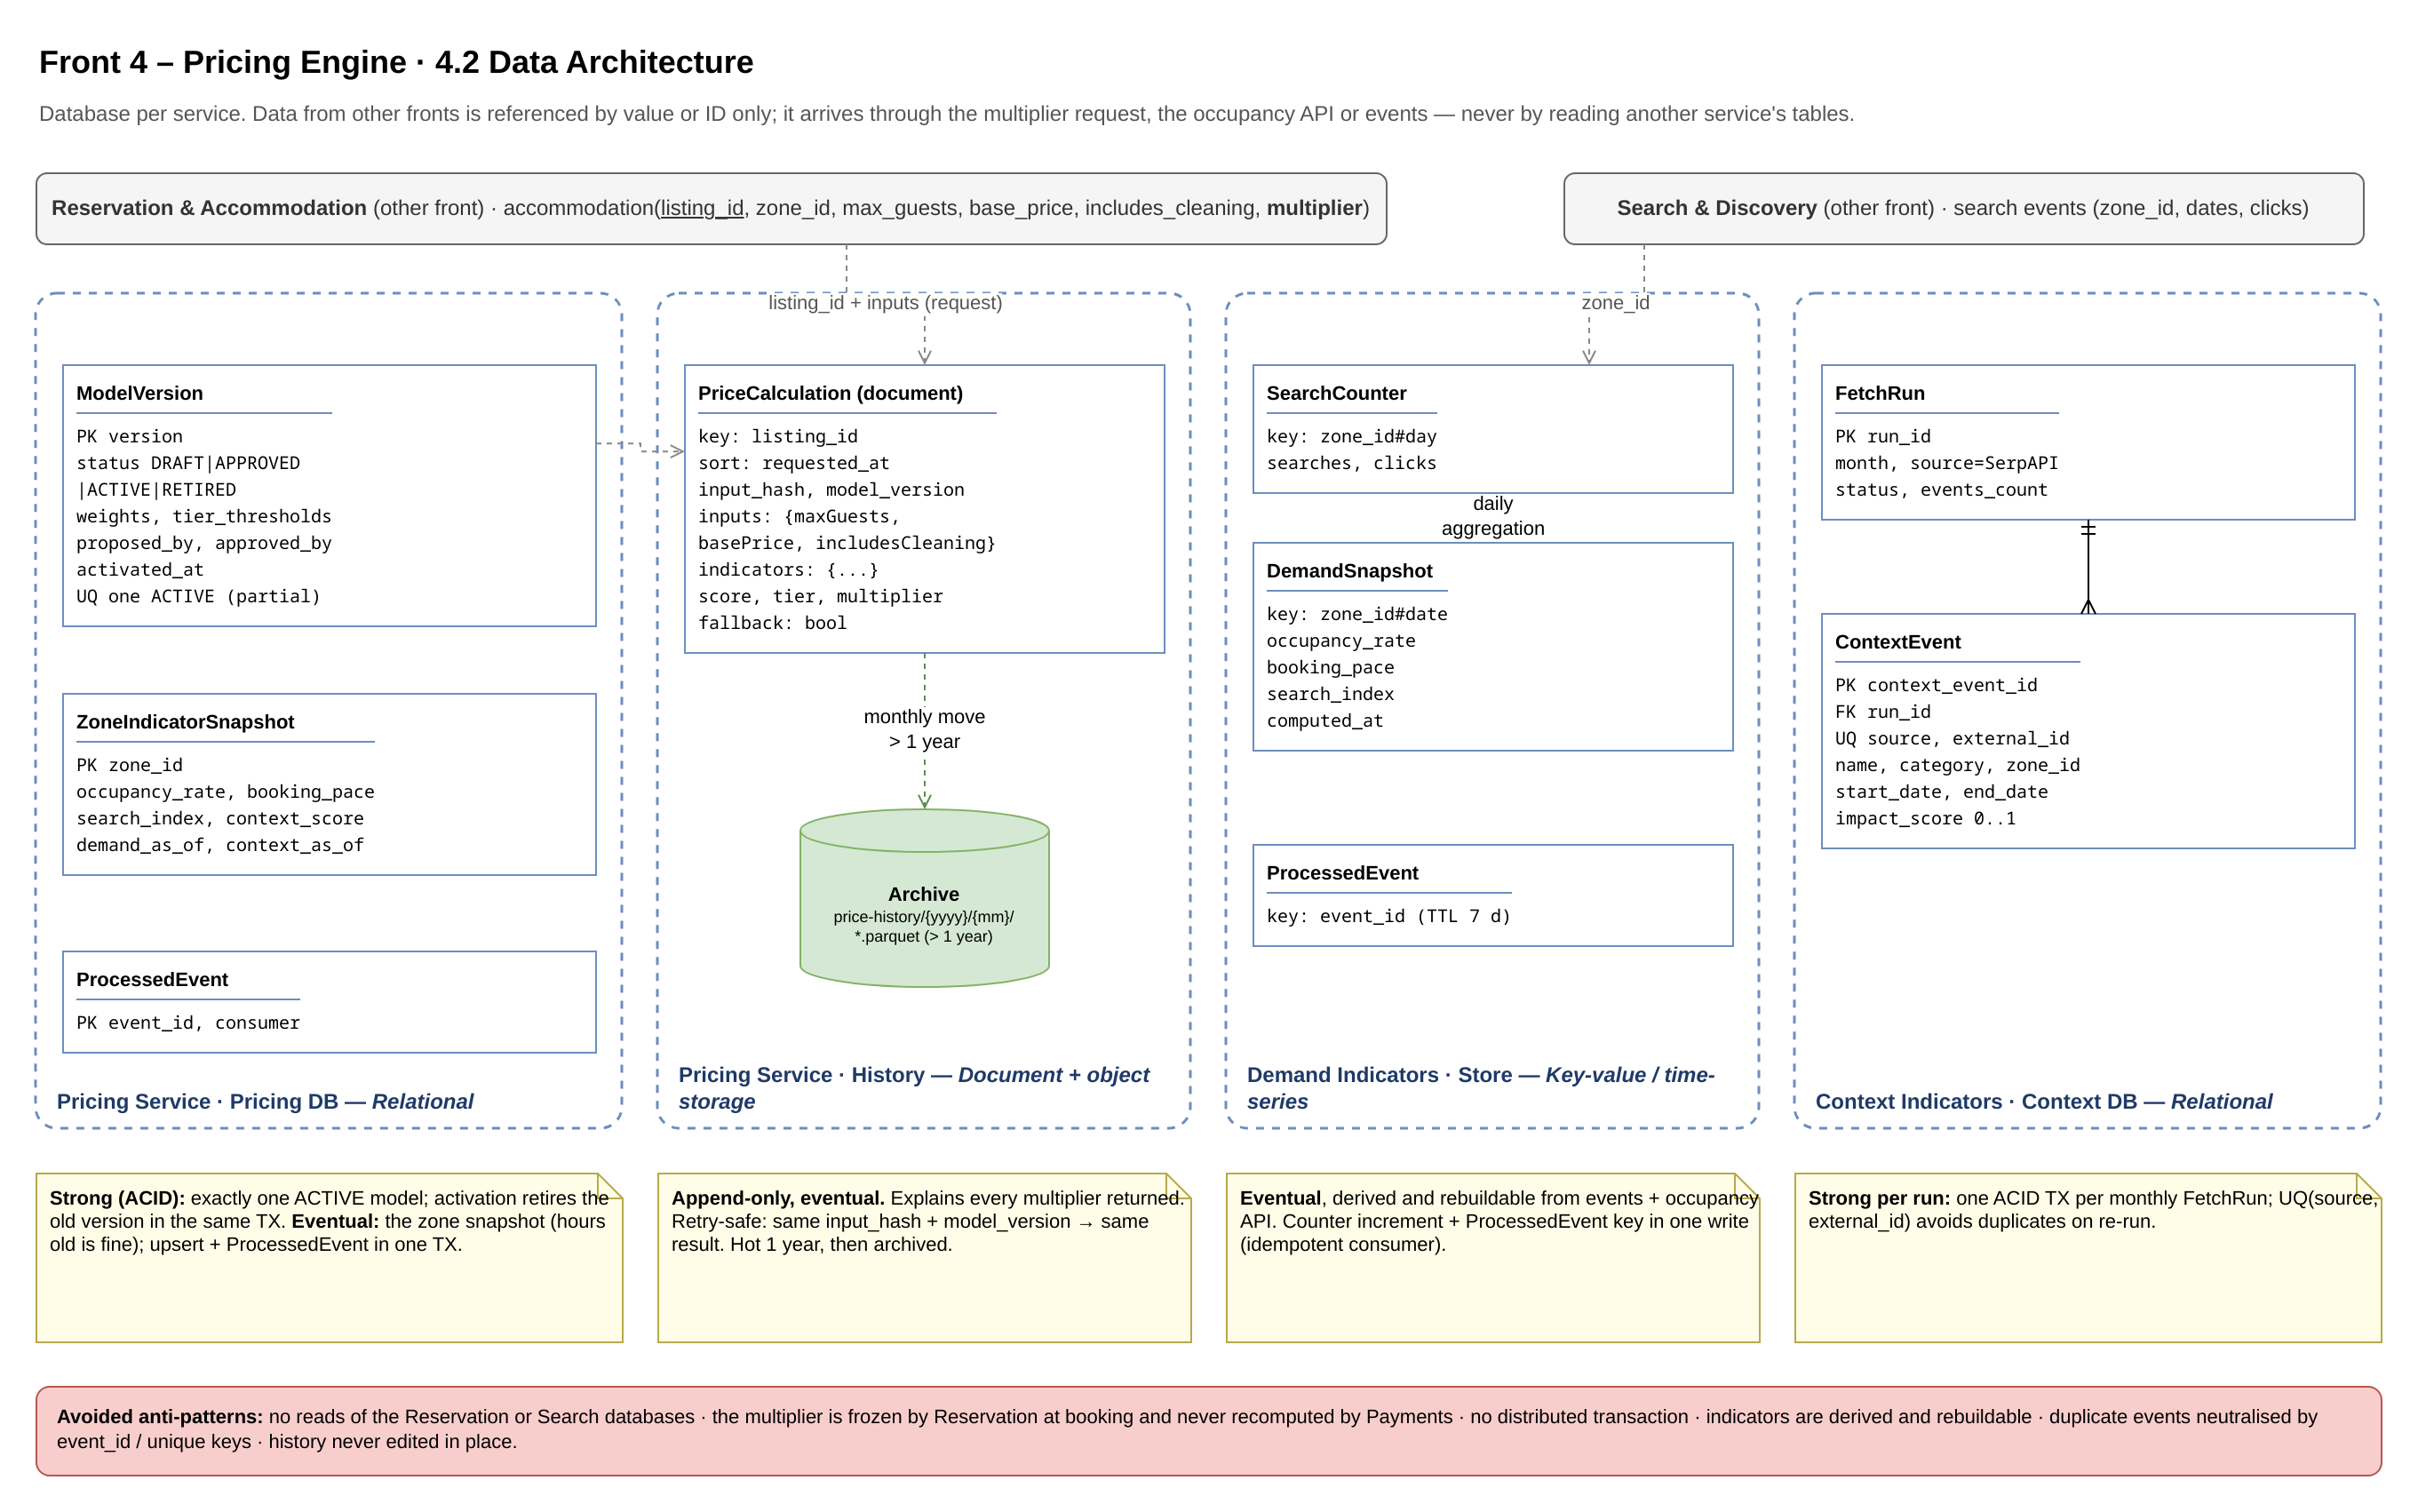
\includegraphics[width=\linewidth]{images/pricing_42_data_architecture.png}
  \caption{Pricing Engine data: owner, storage type and main entities of each
  store. Grey boxes are data of other work streams, referenced by value or
  ID. Source: page 4.2 of \texttt{AirbnbCC.drawio}.}
  \label{fig:price-data}
\end{figure}

\begin{longtable}{@{}L{3.8cm}L{10.0cm}@{}}
\toprule
\textbf{Entity} & \textbf{Main fields and constraints} \\
\midrule
\endhead
\multicolumn{2}{@{}l}{\emph{Pricing DB (Pricing Service, relational)}} \\
\texttt{model\_version} & \texttt{version} (PK), \texttt{status}
  (\texttt{DRAFT}, \texttt{APPROVED}, \texttt{ACTIVE}, \texttt{RETIRED}),
  \texttt{weights}, \texttt{tier\_\allowbreak thresholds}, \texttt{proposed\_by},
  \texttt{approved\_by}, \texttt{activated\_at}; unique partial index on
  \texttt{status = ACTIVE}. \\
\texttt{zone\_\allowbreak indicator\_\allowbreak snapshot} & \texttt{zone\_id} (PK),
  \texttt{occupancy\_\allowbreak rate}, \texttt{booking\_pace}, \texttt{search\_index},
  \texttt{context\_\allowbreak score}, \texttt{demand\_as\_of}, \texttt{context\_as\_of}. \\
\texttt{processed\_event} & (\texttt{event\_id}, \texttt{consumer}) (PK). \\
\addlinespace
\multicolumn{2}{@{}l}{\emph{History (Pricing Service, document store and archive)}} \\
\texttt{PriceCalculation} & Key \texttt{listing\_id}, sort \texttt{requested\_at};
  \texttt{input\_hash}, \texttt{model\_\allowbreak version}, inputs (\texttt{maxGuests},
  \texttt{basePrice}, \texttt{includes\allowbreak Cleaning}), indicators used,
  \texttt{score}, \texttt{tier}, \texttt{multiplier}, \texttt{fallback}. \\
\addlinespace
\multicolumn{2}{@{}l}{\emph{Demand store (Demand Indicators, key-value)}} \\
\texttt{SearchCounter} & Key \texttt{zone\_id\#day}; \texttt{searches}, \texttt{clicks}. \\
\texttt{DemandSnapshot} & Key \texttt{zone\_id\#date}; \texttt{occupancy\_\allowbreak rate},
  \texttt{booking\_pace}, \texttt{search\_index}, \texttt{computed\_at}. \\
\addlinespace
\multicolumn{2}{@{}l}{\emph{Context DB (Context Indicators, relational)}} \\
\texttt{fetch\_run} & \texttt{run\_id} (PK), \texttt{month}, \texttt{source},
  \texttt{status}, \texttt{events\_count}. \\
\texttt{context\_event} & \texttt{context\_\allowbreak event\_id} (PK), \texttt{run\_id} (FK),
  \texttt{source} + \texttt{external\_id} (unique), \texttt{name},
  \texttt{category}, \texttt{zone\_id}, \texttt{start\_date},
  \texttt{end\_date}, \texttt{impact\_\allowbreak score} (0--1). \\
\bottomrule
\caption{Main entities of the Pricing Engine. \texttt{listing\_id} and
\texttt{zone\_id} are logical references to the Reservation and Accommodation
Service (no cross-service foreign keys).}
\label{tab:price-model}
\end{longtable}
\endgroup

% ------------------------- Identity, Communication and Internal Operations -------------------------
\begingroup
\setlength{\emergencystretch}{3em}
\subsubsection{Identity, Communication and Internal Operations}
\label{sec:id-model}

\begin{longtable}{@{}L{3.3cm}L{10.5cm}@{}}
\toprule
\textbf{Store (owner)} & \textbf{Main entities and key fields} \\
\midrule
\endhead
Identity store (Identity \& Access) &
  \texttt{Credential} (\texttt{userId}, \texttt{passwordHash},
  \texttt{status}); \texttt{Session} (\texttt{sessionId}, \texttt{userId},
  \texttt{refreshTokenHash}, \texttt{expiresAt}, \texttt{revokedAt});
  \texttt{MfaFactor}, \texttt{SigningKey}, \texttt{RevocationEntry}. \\
Profile DB (User Profile) &
  \texttt{User} (\texttt{userId}, \texttt{email} unique,
  \texttt{accountStatus}); \texttt{RoleAssignment} (\texttt{userId},
  \texttt{role}, \texttt{grantedBy}, \texttt{reason}); one active role per
  user. \\
Messaging store (Messaging) &
  \texttt{Conversation} (\texttt{conversationId}, \texttt{participantIds},
  \texttt{listingId}); \texttt{Message} (partition
  \texttt{conversationId}, sort \texttt{messageId}; \texttt{senderId},
  \texttt{body}, \texttt{status}); \texttt{ReadState},
  \texttt{Attachment}. \\
Notification store (Notification) &
  \texttt{Notification} (\texttt{eventId}, \texttt{userId},
  \texttt{channel}, \texttt{status}, \texttt{attempts}; unique key
  (\texttt{eventId}, \texttt{userId}, \texttt{channel}));
  \texttt{Notification\allowbreak Preference}, \texttt{Device},
  \texttt{Processed\allowbreak Event}, \texttt{Template}. \\
Support DB (Support) &
  \texttt{SupportCase} (\texttt{caseId}, \texttt{reporterId},
  \texttt{category}, \texttt{relatedReservationId}, \texttt{status},
  \texttt{assigneeId}, \texttt{version}); \texttt{CaseComment};
  \texttt{CaseTransition} (\texttt{fromStatus}, \texttt{toStatus},
  \texttt{actorId}, \texttt{reason}). \\
Administration DB (Administration) &
  \texttt{AdminAction} (\texttt{actionId}, \texttt{actorId},
  \texttt{actionType}, \texttt{targetId}, \texttt{reason},
  \texttt{stepUpVerified}, \texttt{status}); \texttt{Approval};
  \texttt{Policy}. \\
Audit store (Audit) &
  \texttt{AuditRecord} (\texttt{recordId}, \texttt{sequence} unique,
  \texttt{actorId}, \texttt{action}, \texttt{resourceId},
  \texttt{outcome}, \texttt{reason}, \texttt{prevHash},
  \texttt{recordHash}, \texttt{signature}); \texttt{AuditAnchor}
  (\texttt{period}, \texttt{merkleRoot}). \\
\bottomrule
\caption{Main entities of the Identity, Communication and Internal
Operations work stream. \texttt{userId}, \texttt{listingId} and the
\texttt{related*Id} fields are logical references (no cross-service foreign
keys).}
\label{tab:id-model}
\end{longtable}

\paragraph{States.} A message is \texttt{SENT} (stored), \texttt{DELIVERED}
(received by the client) or \texttt{READ}. A notification is \texttt{QUEUED},
\texttt{SENDING}, \texttt{SENT\_\allowbreak TO\_\allowbreak PROVIDER} (accepted by the
provider, not proof of receipt), \texttt{DELIVERED}, \texttt{FAILED} or
\texttt{SUPPRESSED}. A support case is \texttt{OPEN},
\texttt{IN\_\allowbreak PROGRESS}, \texttt{WAITING\_\allowbreak FOR\_\allowbreak USER},
\texttt{RESOLVED} or \texttt{CLOSED}, and every transition is stored with its
actor and reason.

\paragraph{Audit integrity.} Each audit record stores the hash of the previous
one (\texttt{prevHash}) and its own hash, so changing or removing a record
breaks every later hash. A signed anchor (Merkle root of a period) is written
periodically, and an auditor can verify any range.
\endgroup

\subsection{Consistency Requirements}

% ------------------------- Payments and Refunds -------------------------
\begingroup
\setlength{\emergencystretch}{3em}
\subsubsection{Payments and Refunds}
\label{sec:pay-consistency}

\begin{longtable}{@{}L{3.2cm}L{3.6cm}L{7.0cm}@{}}
\toprule
\textbf{Data} & \textbf{Consistency} & \textbf{Why} \\
\midrule
\endhead
Payment state & Strong & A guest must never be charged twice (proposed
  FR11); state reads go to the primary. \\
Never charge twice & Exactly-once effect & Three levels of idempotency:
  caller to Payment Coordination (\texttt{Idempotency-Key}), Payment
  Coordination to gateway (attempt id, stored before the call), and events
  (consumers deduplicate on \texttt{(event\allowbreak Id, consumer)}). \\
Ledger & Strong, append-only & Every transaction balances; a replayed event
  never posts twice (\texttt{source\_\allowbreak event\_\allowbreak id} unique). \\
Reservation, payment and ledger together & Eventual (seconds) & They live in
  different services; agreed through the saga, not one transaction. \\
Gateway & Reconciled & Webhooks plus the 5-minute reconciler; daily
  comparison of the ledger with the gateway settlement report. \\
\bottomrule
\caption{Consistency requirements of Payments and Refunds.}
\label{tab:pay-consistency}
\end{longtable}
\endgroup

\subsubsection{Reservation and Calendar}
\begin{itemize}
  \item \textbf{Strong} for accommodations, calendar and reservations: overlapping
    active entries must be impossible, even under concurrent bookings.
  \item \textbf{Saga} for booking and payment: a reservation is confirmed only
    after a validated payment result; a late payment is recovered or refunded.
  \item \textbf{Eventual} for events, the search index and notifications
    (at-least-once delivery, idempotent consumers).
  \item \textbf{Frozen at booking}: base price, multiplier and conditions are
    copied into the reservation, so later host edits never alter it (FR02).
\end{itemize}

% ------------------------- Pricing Engine -------------------------
\begingroup
\setlength{\emergencystretch}{3em}
\subsubsection{Pricing Engine}
\label{sec:price-consistency}

\begin{longtable}{@{}L{3.4cm}L{3.0cm}L{7.4cm}@{}}
\toprule
\textbf{Data} & \textbf{Consistency} & \textbf{Why} \\
\midrule
\endhead
Active model version & Strong & Two requests must never be priced with
  different active versions at the same time. \\
Zone snapshot and indicators & Eventual (hours) & Demand changes slowly;
  a snapshot of the previous day is accurate enough for a margin tier. \\
Multiplier of a listing & Frozen by Reservation & Stored with the
  accommodation and copied into each reservation; a new model version
  affects only later creates or edits (FR02). \\
Calculation history & Eventual, append-only & Explains past results; never
  edited. \\
\bottomrule
\caption{Consistency requirements of the Pricing Engine.}
\label{tab:price-consistency}
\end{longtable}
\endgroup

% ------------------------- Identity, Communication and Internal Operations -------------------------
\begingroup
\setlength{\emergencystretch}{3em}
\subsubsection{Identity, Communication and Internal Operations}
\label{sec:id-consistency}

\begin{longtable}{@{}L{3.0cm}L{4.4cm}L{6.4cm}@{}}
\toprule
\textbf{Data} & \textbf{Consistency} & \textbf{Why} \\
\midrule
\endhead
Credentials, sessions, revocations & Strong &
  A revoked session or changed password must take effect at once. Token
  claims may be stale only within the short access-token lifetime. \\
Roles and account status & Strong; administrators read their own writes &
  A role change or suspension is a security decision. \\
Messages & Strong per conversation; eventual read state across devices &
  Ordering inside a conversation matters; the read marker of another device
  can lag. \\
Notifications & Eventual &
  A notification is a side effect, not part of the source transaction. \\
Support cases & Strong per case (optimistic concurrency on \texttt{version}) &
  Two agents must not overwrite each other's transition. \\
Administrative actions & Strong locally; the external effect is eventual &
  The action record is local; the change in another service is applied
  through a saga. \\
Audit records & Strong durability on append; the index is eventual &
  Evidence must be durable before the action is confirmed; search can lag. \\
Reservation or payment data used by Support & Eventual (advisory) &
  Read through APIs or events; it may lag and is never edited here. \\
\bottomrule
\caption{Consistency requirements of the Identity, Communication and
Internal Operations work stream.}
\label{tab:id-consistency}
\end{longtable}
\endgroup

\subsection{Transactional Boundaries}

% ------------------------- Payments and Refunds -------------------------
\subsubsection{Payments and Refunds}
\label{sec:pay-boundaries}

\begin{itemize}
  \item \textbf{Inside Payment Coordination (one local transaction):} the
    payment or refund change, its idempotency record and its outbox event
    commit together. The attempt is stored \emph{before} calling the gateway.
  \item \textbf{Inside the Ledger (one local transaction):} one balanced
    journal transaction, its entries and the processed-event mark.
  \item \textbf{Between services (no distributed transaction):} reservation,
    payment and ledger are coordinated by the booking saga. Compensations are
    \emph{void} (hold released, free and immediate) before capture and
    \emph{refund} after capture; a failed refund never undoes a cancellation.
  \item \textbf{With the gateway:} it cannot join any transaction; uncertain
    results stay \texttt{PENDING} and are resolved by webhook or reconciler.
\end{itemize}

\subsubsection{Reservation and Calendar}
Each ACID transaction is local to this service's database:
\begin{itemize}
  \item \textbf{Hold}: release expired holds, insert the \texttt{HOLD} entry and
    the reservation (\texttt{PENDING\_PAYMENT}) and write the outbox event.
  \item \textbf{Confirmation / cancellation / expiration}: conditional
    \texttt{UPDATE} on the expected status, entry conversion or release,
    history and outbox.
  \item \textbf{Listing create or edit}: after the Pricing call (outside the
    transaction), save the accommodation with a \texttt{version} guard and the
    outbox event.
  \item \textbf{Administrative pause}: status change, review flags on future
    reservations and outbox events together.
\end{itemize}
The overlap rule is enforced by the database:
\begin{lstlisting}[language=SQL, basicstyle=\ttfamily\footnotesize, frame=single]
ALTER TABLE calendar_entry ADD CONSTRAINT no_overlap
  EXCLUDE USING gist (listing_id WITH =, period WITH &&)
  WHERE (released_at IS NULL);
\end{lstlisting}

% ------------------------- Pricing Engine -------------------------
\begingroup
\setlength{\emergencystretch}{3em}
\subsubsection{Pricing Engine}
\label{sec:price-boundaries}

\begin{itemize}
  \item \textbf{Multiplier request:} no write transaction; it reads the
    active version and the zone snapshot and appends one history document.
    The same inputs and version produce the same result, so the retry of the
    Reservation Service (one retry within 1.5\,s) is harmless.
  \item \textbf{Model activation (one local transaction):} after the audit
    record is confirmed, the previous \texttt{ACTIVE} version becomes
    \texttt{RETIRED} and the approved one becomes \texttt{ACTIVE}.
  \item \textbf{Indicator events:} the snapshot upsert and the
    processed-event mark commit together.
  \item \textbf{Context run:} one transaction per monthly fetch run.
  \item \textbf{Between services:} storing the multiplier in the listing is
    a transaction of the Reservation Service, outside this work stream; no
    distributed transaction is used.
\end{itemize}
\endgroup

% ------------------------- Identity, Communication and Internal Operations -------------------------
\begingroup
\setlength{\emergencystretch}{3em}
\subsubsection{Identity, Communication and Internal Operations}
\label{sec:id-boundaries}

\begin{itemize}
  \item \textbf{Identity \& Access (one local transaction):} credential
    update and session creation or revocation.
  \item \textbf{User Profile:} profile update, role assignment and outbox
    record.
  \item \textbf{Messaging:} message insert and outbox record, before the
    sender receives the acknowledgement. An attachment is uploaded before the
    message commits; abandoned uploads are cleaned up.
  \item \textbf{Notification:} the duplicate-suppression key and the
    outbound task. A provider failure never rolls back the source operation.
  \item \textbf{Support:} case update, transition record and outbox record.
  \item \textbf{Administration:} action intent, policy decision and outbox
    record.
  \item \textbf{Audit:} each append is atomic and idempotent by
    \texttt{recordId}; the hash-chain order is serialized.
  \item \textbf{Registration (saga):} Identity \& Access creates the
    credential and publishes \texttt{User\allowbreak Registered}; User Profile creates
    the profile. If profile creation fails, the credential stays pending and
    the saga retries or compensates.
  \item \textbf{Administrative action (saga):} authorize, append the
    ``attempt'' record, call the owning service, append the ``outcome''
    record. If the owning service fails, the action is marked
    \texttt{FAILED}, compensated when possible and the operator is notified.
  \item \textbf{Between services:} no distributed transaction; sagas, the
    transactional outbox, idempotency keys and compensation are used.
\end{itemize}
\endgroup

\subsection{Shared Data Anti-patterns Avoided}

% ------------------------- Payments and Refunds -------------------------
\subsubsection{Payments and Refunds}
\label{sec:pay-antipatterns}

\begin{itemize}
  \item \textbf{Shared database:} no other service reads the Payments DB or
    the Ledger DB; they use the APIs and events of this work stream.
  \item \textbf{Recomputing prices:} payments never call Pricing; they use the
    snapshot frozen by the Reservation Service, so the amount charged cannot
    change after booking.
  \item \textbf{Owning other domains' rules:} the cancellation policy stays in
    the Reservation Service and support cases in the Support Service; payments
    only execute the amount requested.
  \item \textbf{Dual writes:} events are published through the outbox.
  \item \textbf{Mutable balances:} balances are derived from append-only
    entries, never updated in place.
  \item \textbf{Sensitive data:} card data is never stored, only the gateway
    token.
\end{itemize}

\subsubsection{Reservation and Calendar}
\begin{itemize}
  \item \textbf{Shared writable database}: no service writes in these tables;
    Pricing reads occupancy through an API.
  \item \textbf{Duplicated authority}: Search keeps a derived index; availability
    is always decided by the calendar.
  \item \textbf{Distributed ACID transaction}: payment is coordinated with
    states, idempotency keys and compensation.
  \item \textbf{Distributed locks}: not used; the exclusion constraint decides.
  \item \textbf{Unbounded event replay}: consumers store processed event IDs.
  \item \textbf{Sensitive payment data}: only gateway references and statuses are stored.
\end{itemize}

% ------------------------- Pricing Engine -------------------------
\begingroup
\setlength{\emergencystretch}{3em}
\subsubsection{Pricing Engine}
\label{sec:price-antipatterns}

\begin{itemize}
  \item \textbf{Shared database:} occupancy is read through the calendar API
    and searches through events, never from the Reservation or Search tables.
  \item \textbf{Recomputing prices:} Payments and Reservation use the frozen
    multiplier; the engine never changes the price of an existing booking.
  \item \textbf{Synchronous fan-out:} the request does not call the indicator
    services or SerpAPI; it reads a local snapshot fed by events.
  \item \textbf{Duplicated authority:} the zone snapshot is a derived copy;
    the indicator services remain the owners and it can be rebuilt from them.
  \item \textbf{Mutable history:} calculations are appended, never updated.
\end{itemize}
\endgroup

% ------------------------- Identity, Communication and Internal Operations -------------------------
\begingroup
\setlength{\emergencystretch}{3em}
\subsubsection{Identity, Communication and Internal Operations}
\label{sec:id-antipatterns}

\begin{itemize}
  \item \textbf{Shared database:} each service has its own store and
    credentials; there are no cross-service joins or direct table access.
    Other services use the APIs and events of this work stream.
  \item \textbf{Dual writes:} state changes and event publication are bound
    by the transactional outbox.
  \item \textbf{Shared cache as source of truth:} caches (roles, contact
    data, public keys) are read-through projections with explicit
    invalidation; the authoritative data stays in the owner.
  \item \textbf{Distributed transactions:} cross-service workflows use sagas,
    idempotency keys and compensation instead of two-phase commit.
  \item \textbf{Audit in mutable logs:} operational logs are not evidence;
    audit records are append-only, hash-chained and immutable.
  \item \textbf{Copies of owned data in events:} \texttt{Message\allowbreak Created}
    carries identifiers and metadata, not the message body; the profile is
    read from User Profile, not copied.
  \item \textbf{Duplicate notifications:} consumers store processed event
    identifiers and apply a key per event, user and channel.
\end{itemize}

\paragraph{Security and privacy controls.}
\begin{itemize}
  \item TLS protects client-to-service and service-to-service traffic; data
    is encrypted at rest, and keys and third-party credentials live in
    dedicated key and secret stores, not in configuration.
  \item Each service identity can call only the APIs and publish or consume
    only the events it needs (least privilege).
  \item Access tokens are short-lived, refresh tokens are rotated, and a role
    change or suspension revokes the sessions of the user.
  \item Administrator, auditor and support roles require MFA; sensitive
    administrative actions also need a fresh step-up verification and a
    documented reason.
  \item Passwords, tokens, full message bodies and complete payment data are
    excluded from logs and audit payloads.
\end{itemize}
\endgroup

